\documentclass[a4paper]{article}
%\usepackage[singlespacing]{setspace}
\usepackage[onehalfspacing]{setspace}
%\usepackage[doublespacing]{setspace}
\usepackage{geometry} % Required for adjusting page dimensions and margins
\usepackage{amsmath,amsfonts,stmaryrd,amssymb,mathtools,dsfont} % Math packages
\usepackage{tabularx}
\usepackage{colortbl}
\usepackage{listings}
\usepackage{amsmath}
\usepackage{amssymb}
\usepackage{amsthm}
\usepackage{subcaption}
\usepackage{float}
\usepackage[table,xcdraw]{xcolor}
\usepackage{tikz-qtree}
\usepackage{forest}
\usepackage{changepage,titlesec,fancyhdr} % For styling Header and Titles
\usepackage{amsmath}
\pagestyle{fancy}
\usepackage{diagbox}
\usepackage{xfrac}
\usepackage{pgfplots}
\pgfplotsset{compat=1.18}

\usepackage{enumerate} % Custom item numbers for enumerations
\usepackage{enumitem}

\usepackage[ruled]{algorithm2e} % Algorithms

\usepackage{hyperref}

\usepackage[framemethod=tikz]{mdframed} % Allows defining custom boxed/framed environments

\usepackage{listings} % File listings, with syntax highlighting
\lstset{
	basicstyle=\ttfamily, % Typeset listings in monospace font
}

\usepackage[ddmmyyyy]{datetime}


\geometry{
	paper=a4paper, % Paper size, change to letterpaper for US letter size
	top=2.5cm, % Top margin
	bottom=3cm, % Bottom margin
	left=2.5cm, % Left margin
	right=2.5cm, % Right margin
	headheight=25pt, % Header height
	footskip=1.5cm, % Space from the bottom margin to the baseline of the footer
	headsep=1cm, % Space from the top margin to the baseline of the header
	%showframe, % Uncomment to show how the type block is set on the page
}
\lhead{Stochastik für die Informatik\\Wintersemester 2024/2025}
\chead{\bfseries{Übungsblatt 13}\\}
\rhead{Lienkamp, 8128180\\Werner, 7987847}
\begin{document}
\setcounter{section}{13}
\subsection{$\mathcal{X}^2$-Verteilung}
Für den Zeitraum von 1999 bis 2009 wurde gezählt, wieviele Filme pro Jahr mit Nicolas Cage erschienen sind und wieviel Menschen im jeweiligen Jahr in den USA durch Ertrinken in einem Pool umgekommen sind. Das ergab die folgenden Zahlen:\\
\begin{table}[ht]
\centering
\begin{tabular}{l|c|c|c|c}
\diagbox{Ertrunkene}{Cage-Filme } & 1 & 2 & 3 & 4 \\ \hline
90-100 & 3 & 1 & 2 & 0 \\
101-110 & 0 & 3 & 0 & 1 \\
111-120 & 0 & 0 & 0 & 1\\
\end{tabular}
\end{table}\\
Berechnen Sie den p-Wert für das Testproblem\\
\hspace*{2cm} H0 : Anzahl Filme und Anzahl Todesfälle sind unabhängig \hspace*{0.5cm} gegen\\
\hspace*{2cm} H1 : Anzahl Filme und Anzahl Todesfälle sind nicht unabhängig.\\
Was ist das Ergebnis des Tests zum Signifikanzniveau $\alpha = 0.1$ bzw. $\alpha = 0.05$?\\\\
\subsection{Wettermodell}
Das Wetter an einem Tag sei durch einen der beiden Zustände "sonnig" und "regnerisch" beschrieben und entwickle sich nach den nachfolgend beschriebenen Regeln.\\\\
(a) Das Wetter von morgen hängt vom Wetter von heute und gestern ab. Hat es gestern und heute geregnet, so regnet es morgen mit Wahrscheinlichkeit $\sfrac{1}{2}$; regnet es heute, aber gestern nicht, so regnet es morgen mit Wahrscheinlichkeit $\sfrac{6}{10}$; regnete es gestern, aber heute nicht, so regnet es morgen mit Wahrscheinlichkeit $\sfrac{4}{10}$; und regnete es nicht, so regnet es morgen mit Wahrscheinlichkeit $\sfrac{1}{5}$.
Geben Sie einen geeigneten Zustandsraum, den Übergangsgraphen und die Übergangswahrscheinlichkeiten an.\\\\
(b) Berechnen Sie für dieses Modell die Wahrscheinlichkeit, dass es am Freitag nicht regnen wird, wenn es Dienstag und Mittwoch geregnet hat.\\\\
\subsection{}
Ein Server verarbeitet Client anfragen. Dabei kommt es durch Übertragungsfehler zu fehlerhaften Anfragen. Im Falle einer fehlerhaften Anfrage des Clients fordert der Server den Client auf die Anfrage erneut zu senden. Sollten 5 fehlerhafte Anfragen hintereinander eingehen unterbricht der Server die Verbindung zum Client. Wir gehen der Einfachheit halber davon aus, dass alle Anfragen (auch die mehrfach Anfragen des selben Clients) unabhängig voneinander mit Wahrscheinlichkeit $p$ fehlerhaft sind. Bestimmen Sie die erwartete Anzahl an Anfragen, bis
der Server das erste mal eine Verbindung abbricht.\\
\textit{Hinweis:} Nutzen Sie zur Modellierung eine irreduzible und aperiodische Markovkette. Außerdem sollten Sie Satz 11.8 aus dem Buch verwenden.\\\\
\subsection{(Irreduzibilität und Aperiodizität)}
(a) Welche der Markovketten zu den folgenden Übergangsgraphen sind irreduzibel bzw. aperiodisch? Begründen Sie Ihre Aussage!\\
\begin{figure}[H]
    \centering
    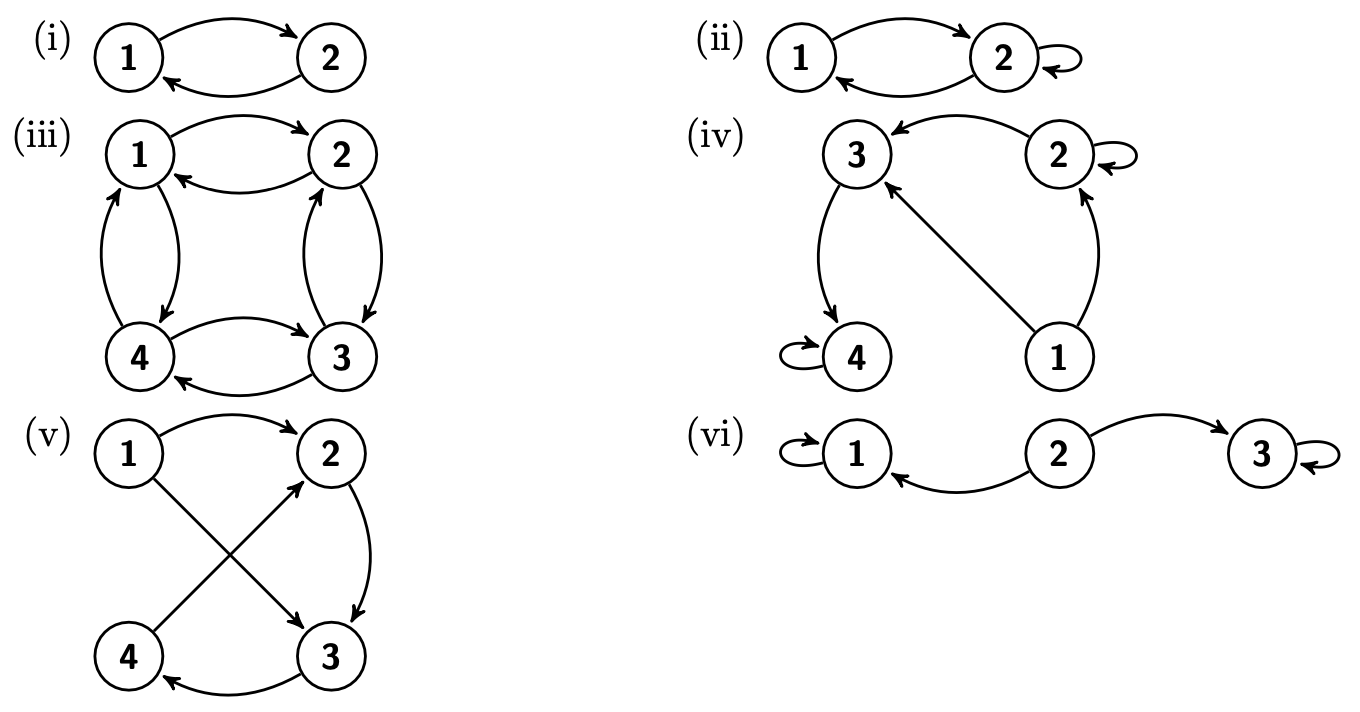
\includegraphics[width=0.8\linewidth]{markov.png}
\end{figure}
\noindent (b) Betrachten Sie alle die Markovketten in der Teilaufgabe (a), die irreduzibel sind. Welche von diesen Ketten konvergieren gegen ihre eindeutige invariante Verteilung, gegeben, dass sie vom jeweiligen Zustand 1 starten?\\\\
(c) Zeigen Sie, dass die Markovkette zum Übergangsgraphen (vi) unendlich viele invariante Verteilungen hat.\\\\

\textbf{Hinweise zur Bearbeitung der Aufgaben:}
\begin{itemize}
    \item Die Hausaufgabenblätter werden Freitags auf Moodle veröffentlicht und enthalten Hausaufgaben, die in der darauf folgenden Woche entweder \textbf{vor der Vorlesung am Freitag um 12:00} Uhr in Hörsaal V abzugeben sind oder \textbf{vor Freitag 12:00 Uhr} in das Schließfach Ihres Tutors (Robert-Mayer-Straße 6-8, 3. Stock) eingeworfen werden müssen.
    \item Die Hausaufgaben werden anschließend in den Tutorien der nächsten Woche besprochen.
\end{itemize}
\end{document}
